\documentclass[10pt]{article}
\usepackage[ngerman]{babel}
\usepackage[utf8]{inputenc}
\usepackage[T1]{fontenc}
\usepackage{graphicx}
\usepackage[export]{adjustbox}
\graphicspath{ {./images/} }
\usepackage{amsmath}
\usepackage{amsfonts}
\usepackage{amssymb}
\usepackage[version=4]{mhchem}
\usepackage{stmaryrd}

\title{Bachelor of Science (BSc) in Informatik \\
 Modul Software-Entwicklung 1 (SWEN1) }

\author{}
\date{}


\begin{document}
\maketitle
\section*{LE 04 - Domänenmodellierung}
SWEN1/PM3 Team:\\
R. Ferri (feit), D. Liebhart (lieh), K. Bleisch (bles), G. Wyder (wydg)

\section*{Um was geht es?}
\begin{itemize}
  \item Anforderungen können besser verstanden und umgesetzt werden, wenn man eine klare Vorstellung von der Fachdomäne hat.
  \item Die Erfahrung hat gezeigt, dass es eine gute Wahl ist, wenn die Software so strukturiert wird wie die Fachdomäne.
  \item Die statischen Aspekte einer Fachdomäne können mit einem vereinfachten Klassendiagramm modelliert werden.
\end{itemize}

\section*{Lernziele LE 04 - Domänenmodellierung}
Sie sind in der Lage:

\begin{itemize}
  \item Ein vereinfachtes UML-Klassendiagramm zu zeichnen,
  \item Ein Modell der Fachdomäne in Form eines UML-Klassendiagramms zu erstellen,
  \item Konzepte der Fachdomäne in Anforderungen zu identifizieren, in Beziehung zueinander zu setzen und mit sinnvollen Attributen zu versehen,
  \item Beschreibungskonzepte, Generalisierungen/Spezialisierungen, Kompositionen, Rollen und Assoziationsklassen zu identifizieren und korrekt in UML abzubilden.
\end{itemize}

\section*{Agenda}
\begin{enumerate}
  \item Einleitung und Motivation
  \item Grundlagen
  \item Vorgehen
  \item Analyse Muster
  \item Wrap-up und Ausblick
\end{enumerate}

\section*{Zur Erinnerung: Auslosungstool}
School of\\
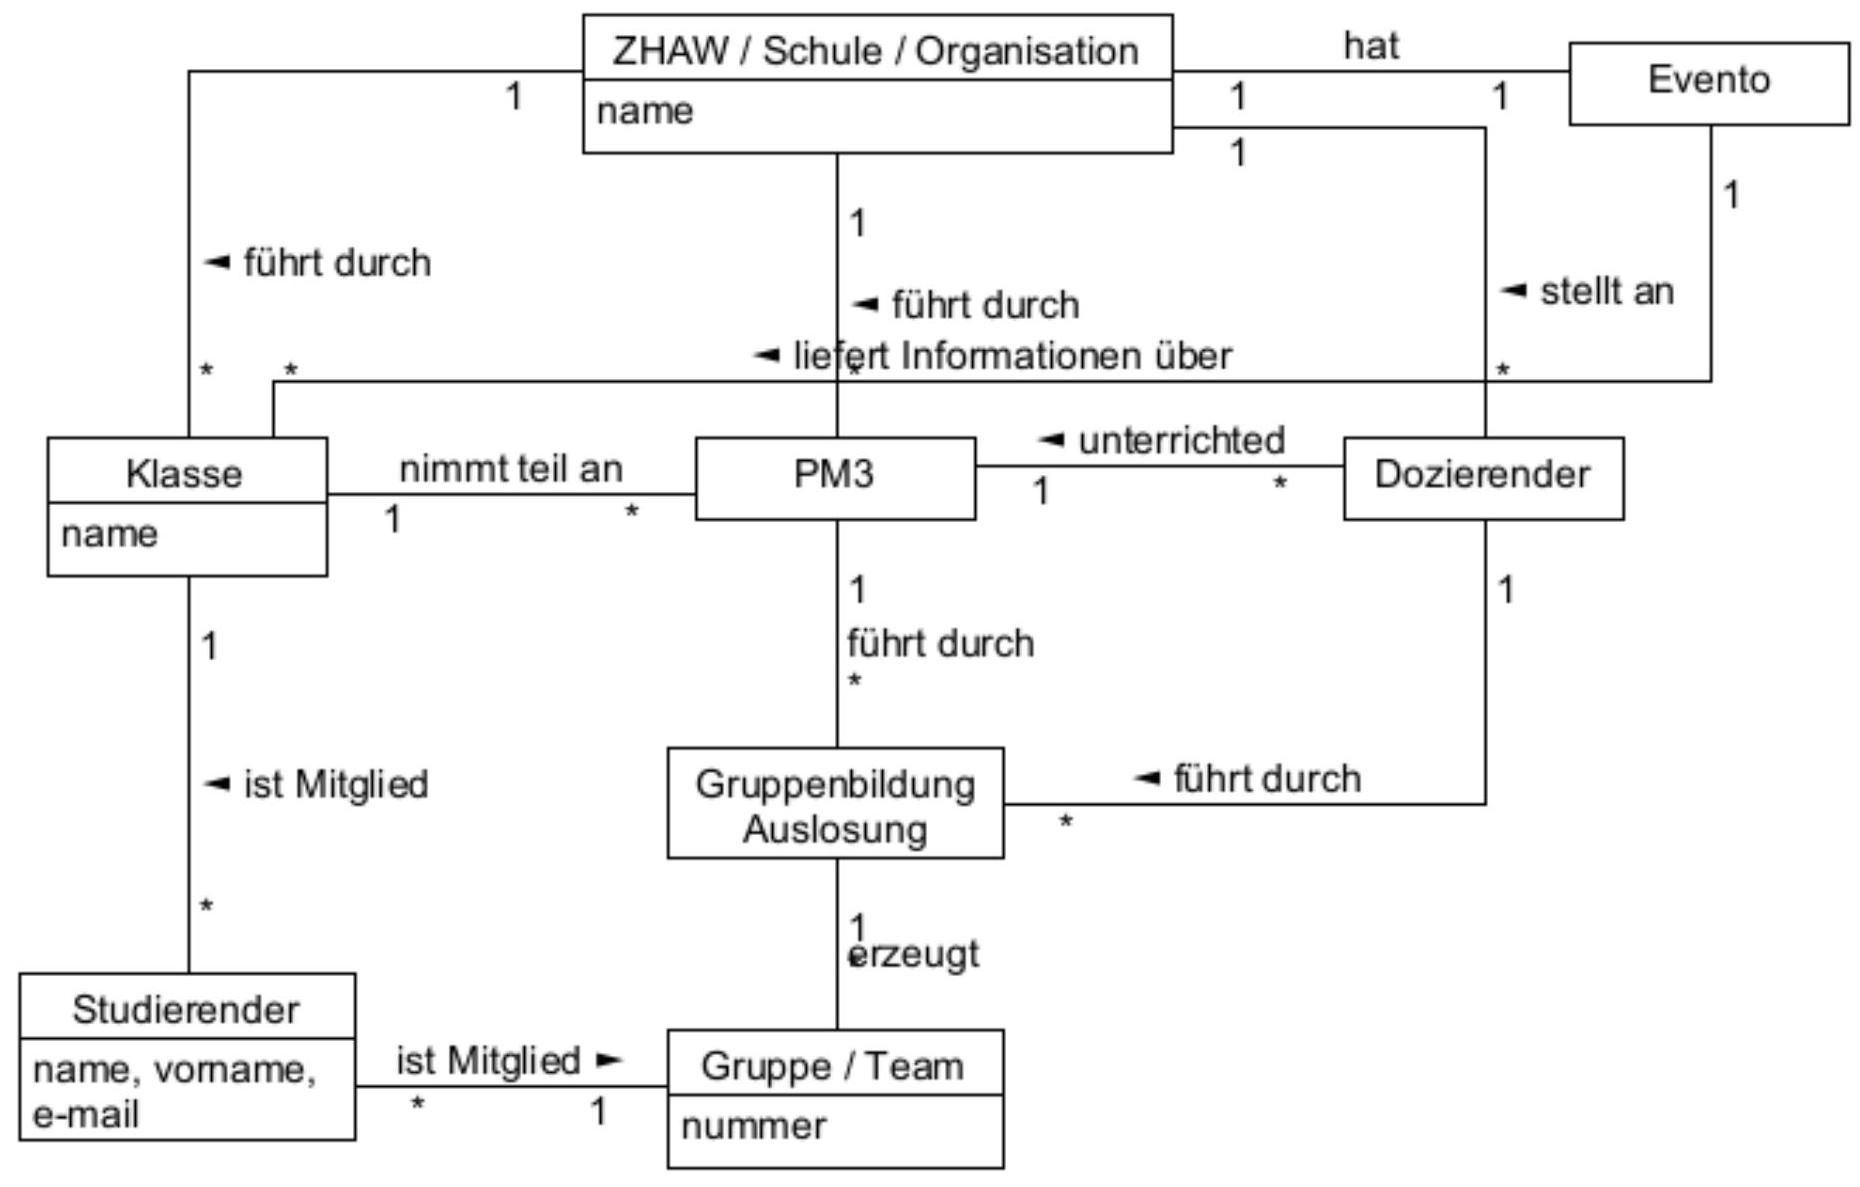
\includegraphics[max width=\textwidth, center]{2025_01_02_5d799754d4e57e7473c6g-05}

\section*{Zur Erinnerung: Auslosungstool}
School of\\
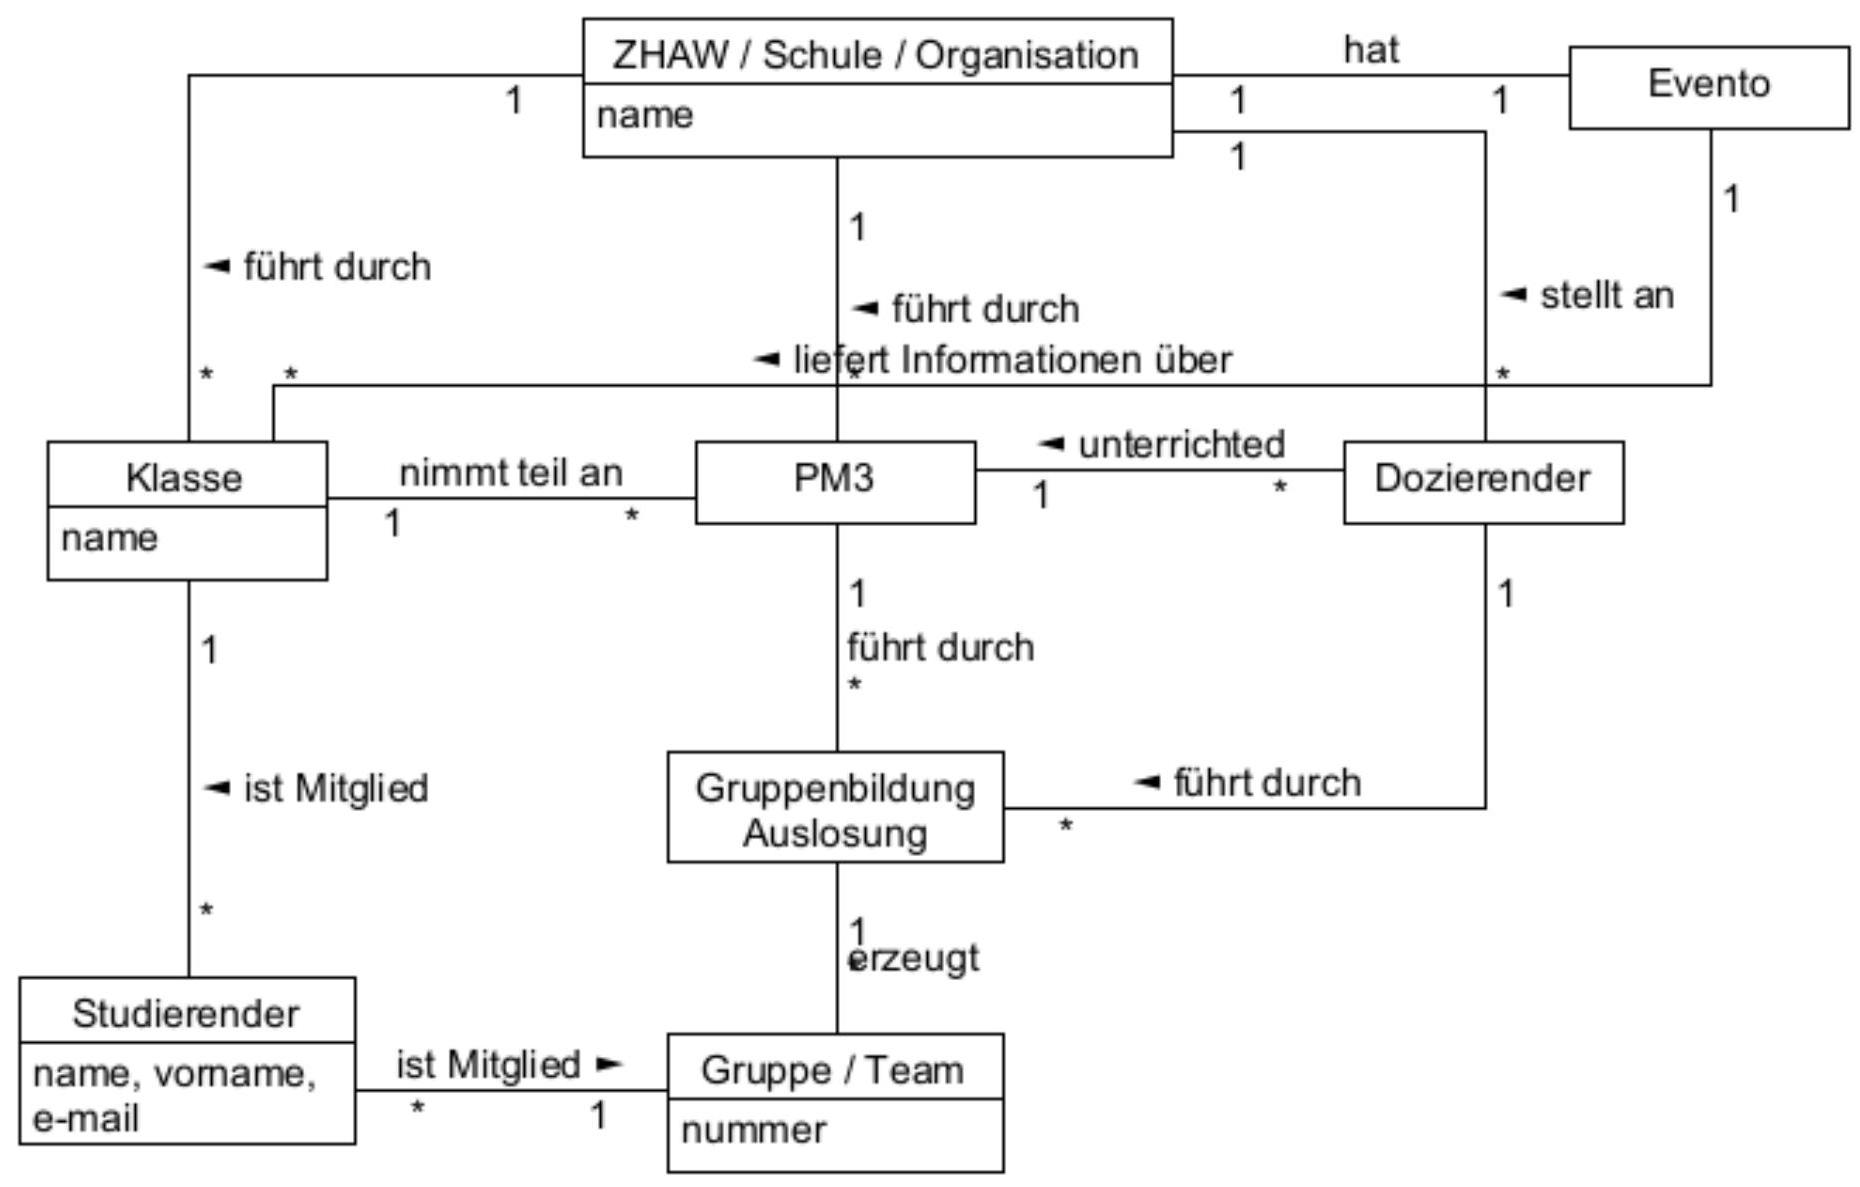
\includegraphics[max width=\textwidth, center]{2025_01_02_5d799754d4e57e7473c6g-06}

\section*{Agenda}
\begin{enumerate}
  \item Einleitung und Motivation
  \item Grundlagen
  \item Vorgehen
  \item Analyse Muster
  \item Wrap-up und Ausblick
\end{enumerate}

\section*{Domänenmodell als vereinfachtes UML Klassendiagramm}
School of Engineering

\begin{itemize}
  \item Das Domänenmodell wird als UML
\end{itemize}

Klassendiagramm in einer vereinfachten\\
Form gezeichnet.

\begin{itemize}
  \item Konzepte werden als Klassen modelliert.
  \item Eigenschaften von Konzepten werden mit Attributen modelliert. Die Typangabe entfällt üblicherweise.
  \item Assoziationen werden verwendet, um Beziehungen zwischen Konzepten zu modellieren. Dabei beschreibt der Name der Assoziation die Beziehung und an beiden Enden werden Multiplizitäten angeschrieben.\\
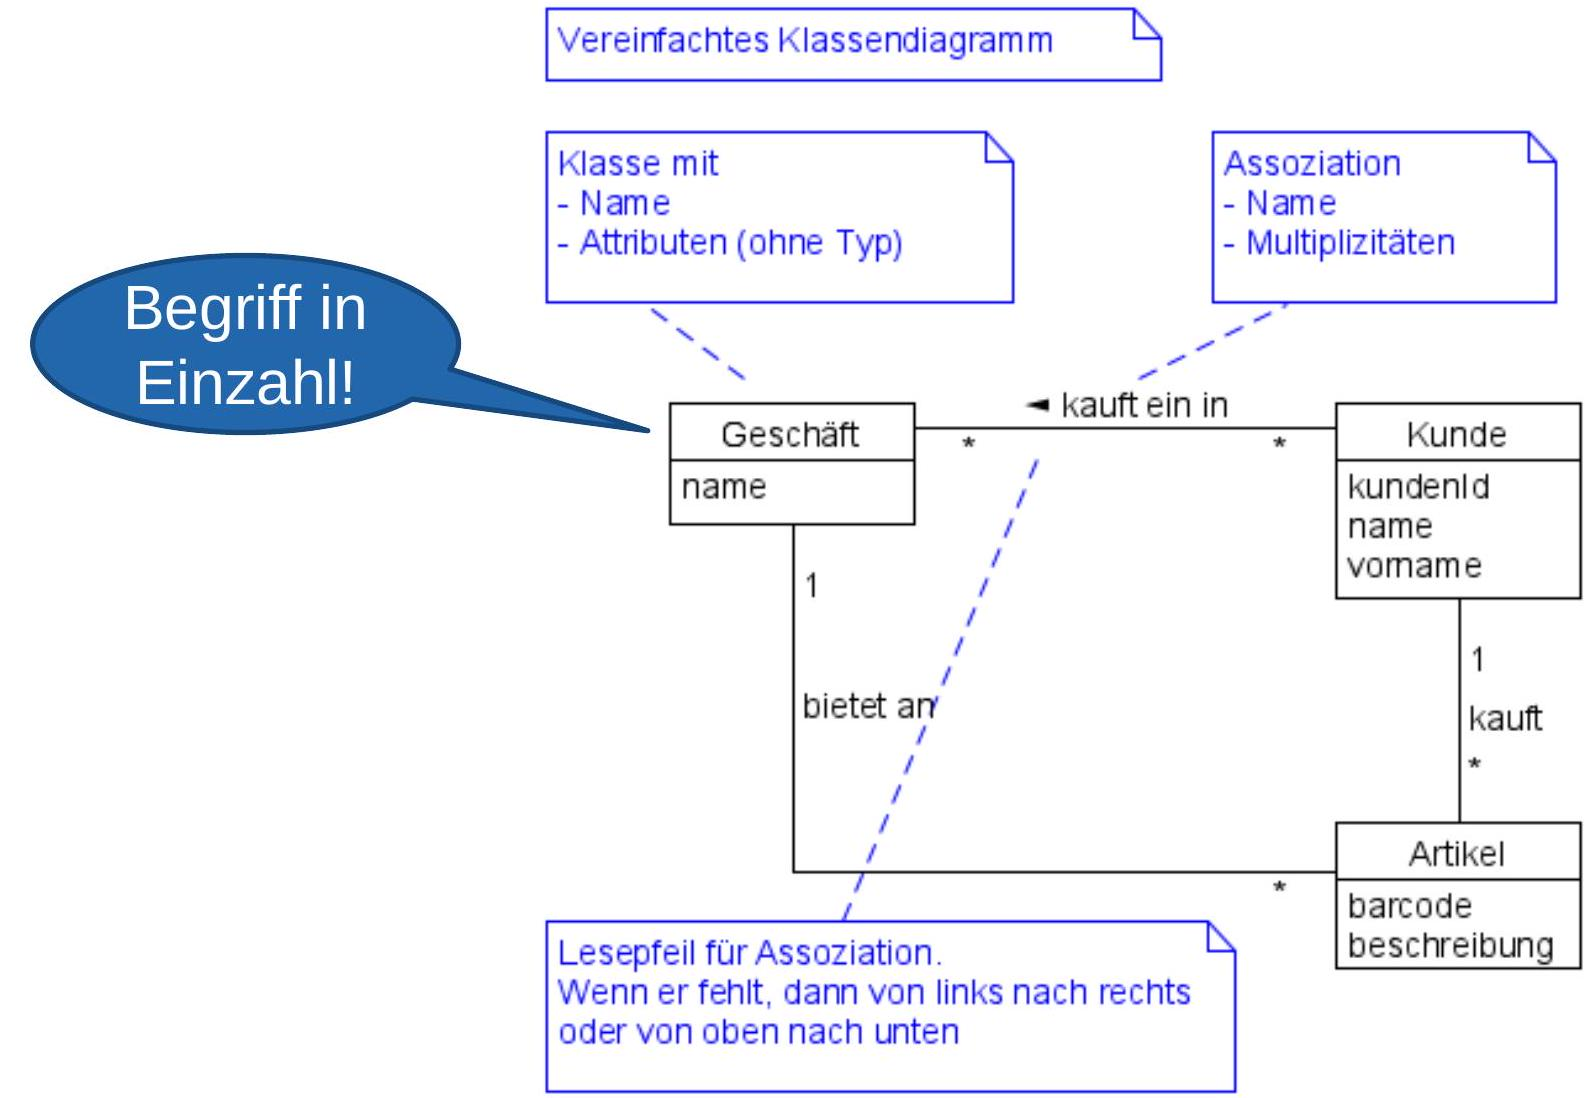
\includegraphics[max width=\textwidth, center]{2025_01_02_5d799754d4e57e7473c6g-08}
\end{itemize}

\section*{Agenda}
\begin{enumerate}
  \item Einleitung und Motivation
  \item Grundlagen
  \item Vorgehen
  \item Analyse Muster
  \item Wrap-up und Ausblick
\end{enumerate}

\section*{Vorgehen}
\begin{itemize}
  \item Zuerst werden die Konzepte identifiziert
  \item Eigenes oder fremdes Fachwissen und Erfahrung verwenden
  \item Substantive aus Anwendungsfällen herausziehen
  \item Kategorienliste verwenden
\end{itemize}

\section*{Vorgehen}
\begin{itemize}
  \item Zuerst werden die Konzepte identifiziert
  \item Eigenes oder fremdes Fachwissen und Erfahrung verwenden
  \item Substantive aus Anwendungsfällen herausziehen
  \item Kategorienliste verwenden
  \item Konzepte mit Attributen versehen
  \item Fachwissen
  \item Konzepte in Verbindung zueinander setzen
  \item Fachwissen
  \item Kategorienliste verwenden
  \item Dabei Auftraggeber und/oder Fachexperten beiziehen
  \item Vorgehensweise eines Kartografen anwenden
\end{itemize}

\section*{Datentypen von Attributen}
\begin{itemize}
  \item Die meisten Attributtypen sind einfach («primitiv»).
  \item Integer, float, boolean
  \item Werden im DM normalerweise nicht angegeben
  \item Attributtypen können auch zusammengesetzte Typen sein
  \item Nur ihr Inhalt und nicht ihre Identität ist relevant.
  \item Die Java Typen String und Instant sind solche Typen.
  \item Vergleich mit equals (...) und nicht mit ==
\end{itemize}

\section*{Anti-Pattern: Attribute an Stelle von Assoziationen}
\begin{itemize}
  \item Verwenden Sie Assoziationen und nicht Attribute, um Konzepte in Beziehung zueinander zu setzen.\\
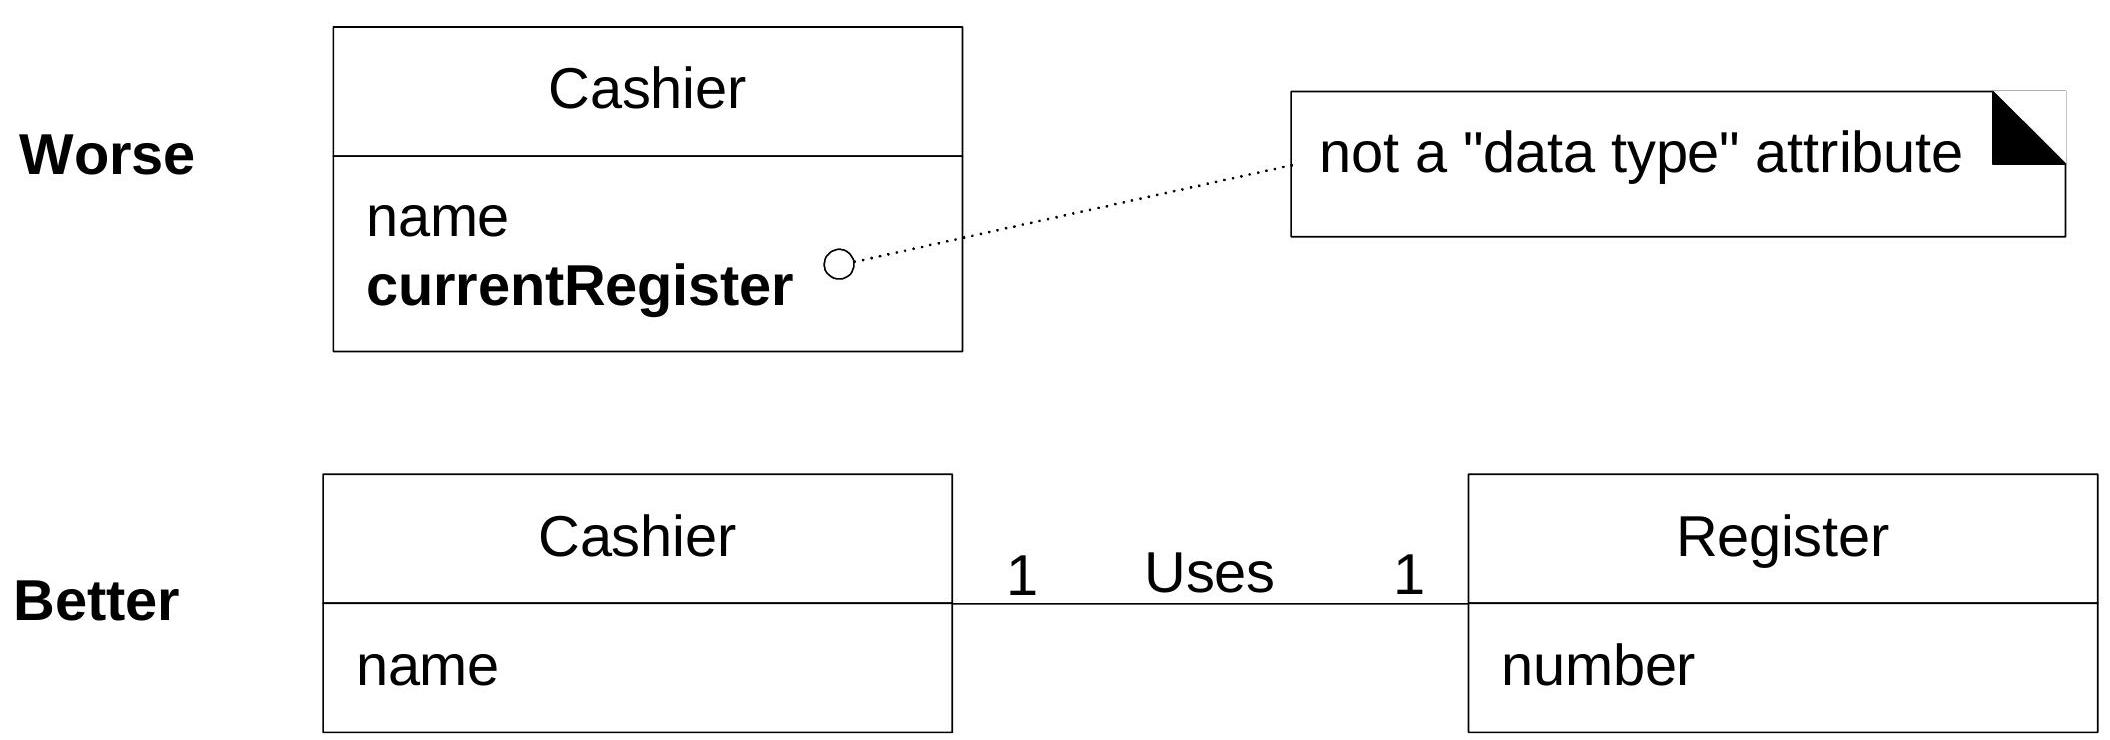
\includegraphics[max width=\textwidth, center]{2025_01_02_5d799754d4e57e7473c6g-13}
\end{itemize}

\section*{Anti-Pattern : Software-Klassen}
School of\\
Engineering\\
InIT Institut für angewandte Informationstechnologie

\begin{itemize}
  \item Keine Software Klassen im Domänenmodell, die es so nicht in der Fachdomäne gibt.\\
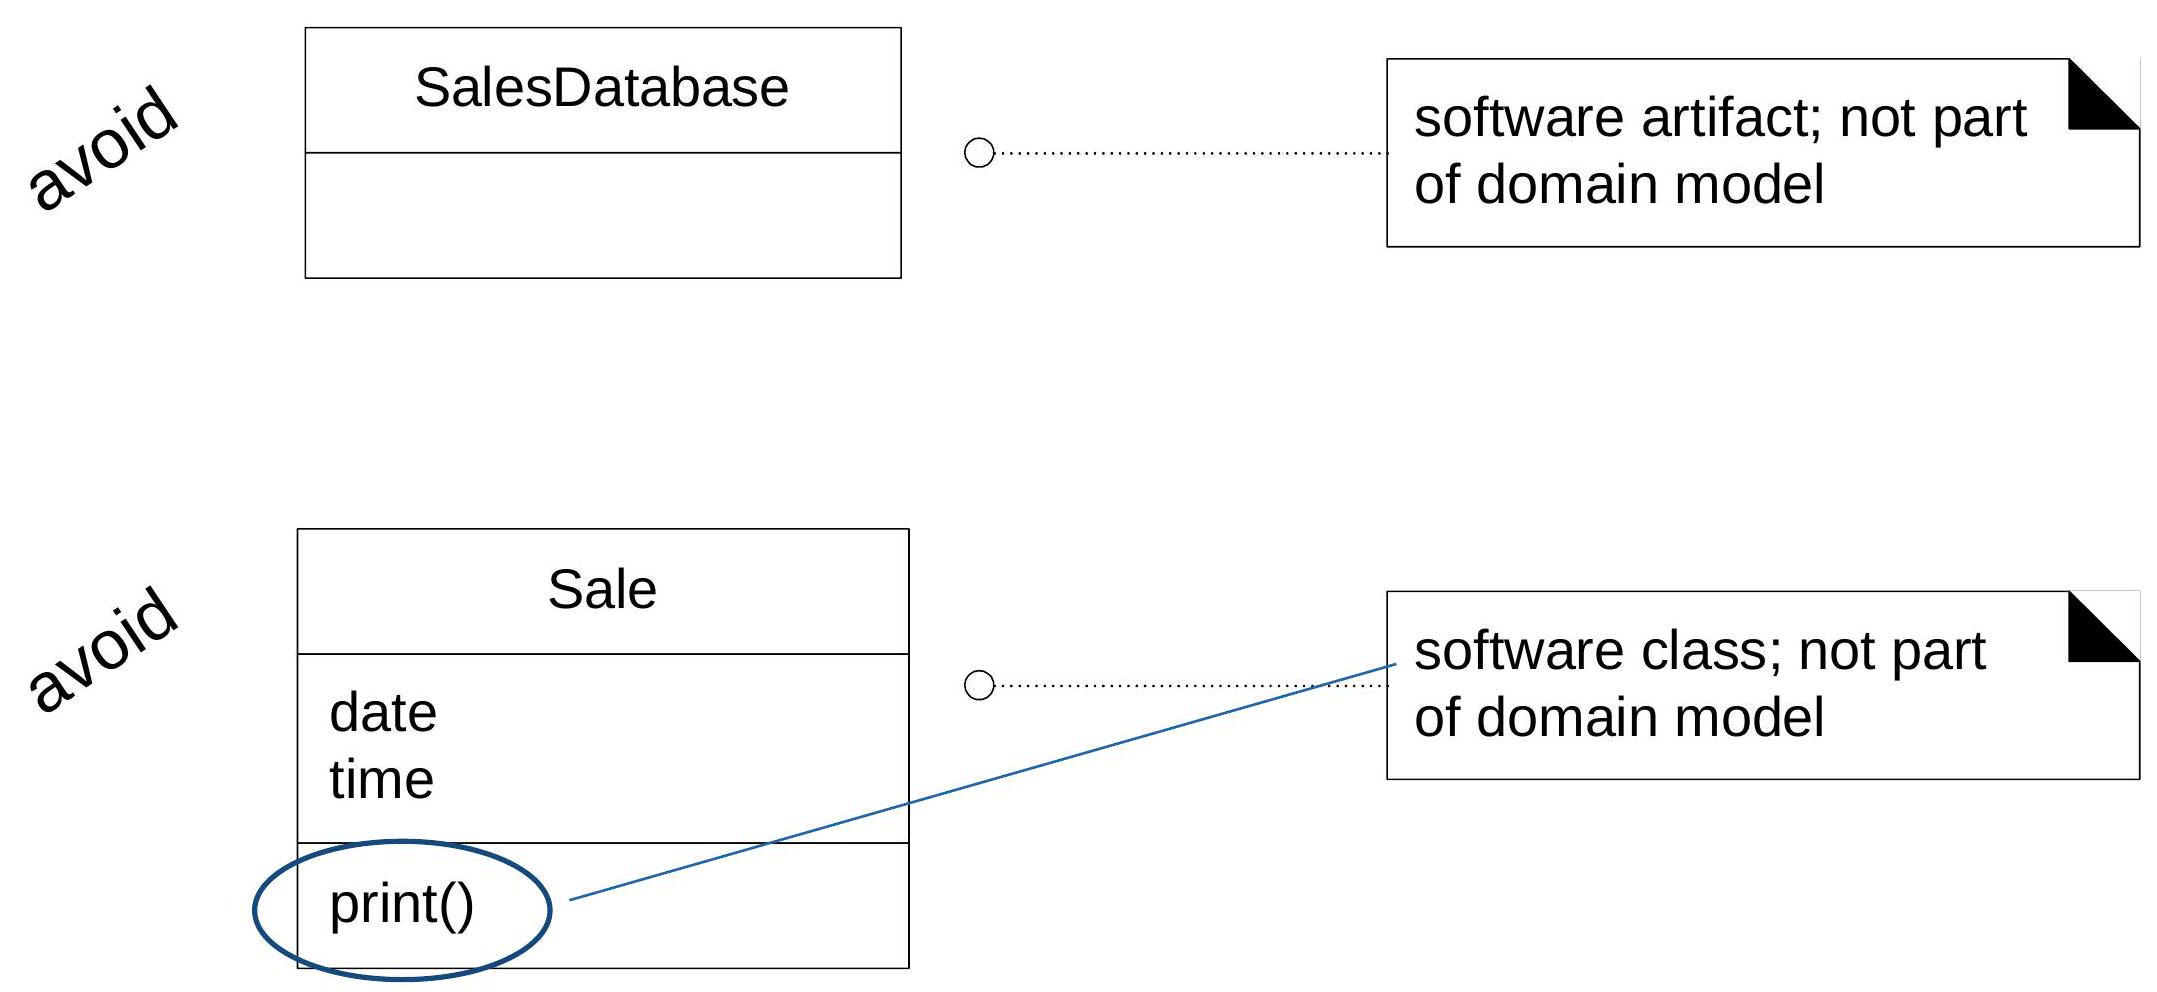
\includegraphics[max width=\textwidth, center]{2025_01_02_5d799754d4e57e7473c6g-14}
\end{itemize}

\section*{Ein paar Bemerkungen zur Domänenmodellierung}
\begin{itemize}
  \item Das perfekte Domänenmodell gibt es so nicht.
  \item Es ist immer eine Annäherung an den Fachbereich.
  \item Werkzeug fürs
  \item Verstehen der Fachdomäne
  \item Kommunikation im Team und mit dem Auftraggeber
\end{itemize}

\section*{Domänenmodell für die elektronische Kasse}
\begin{center}
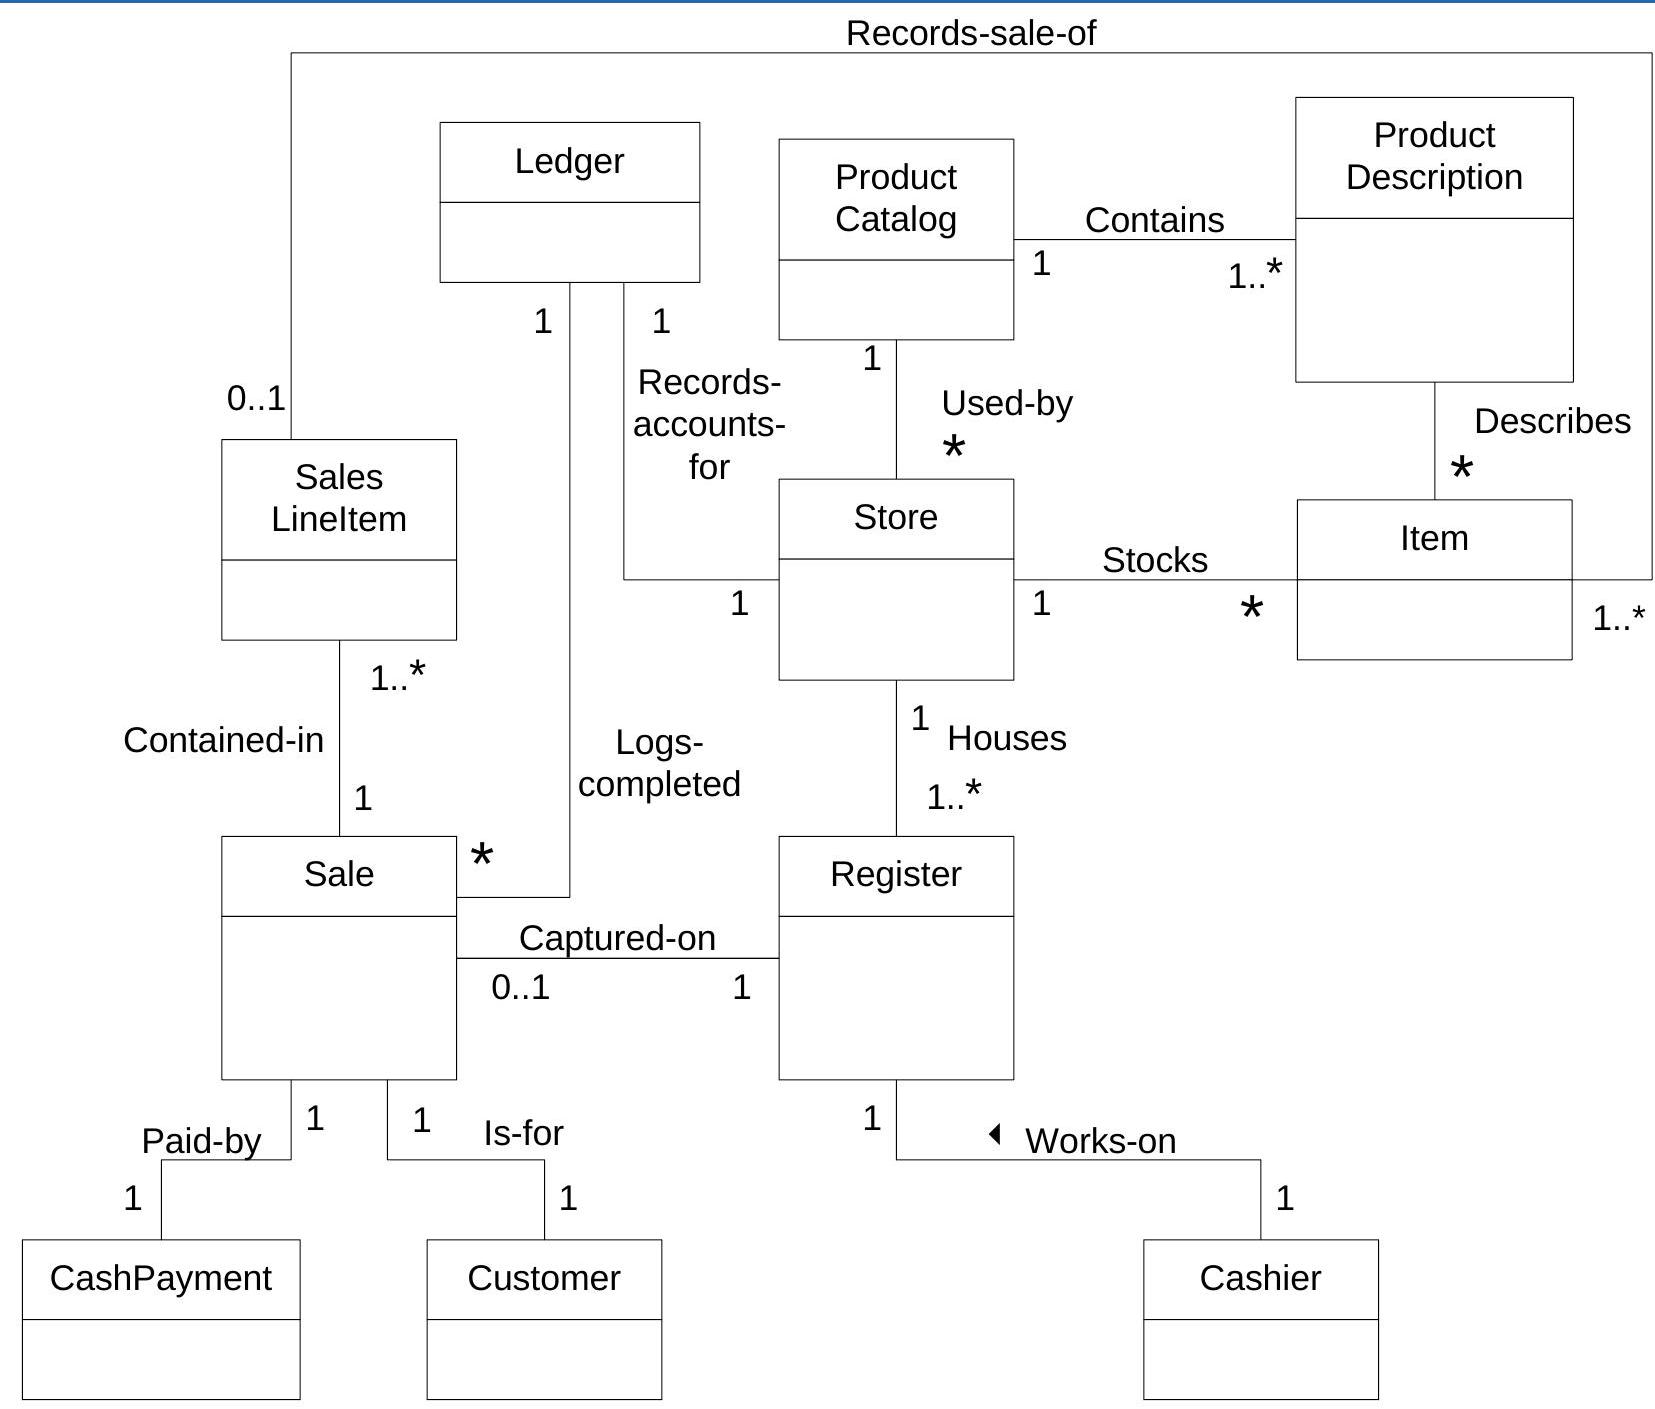
\includegraphics[max width=\textwidth]{2025_01_02_5d799754d4e57e7473c6g-16}
\end{center}

\section*{Agenda}
\begin{enumerate}
  \item Einleitung und Motivation
  \item Grundlagen
  \item Vorgehen
  \item Analysemuster
  \item Wrap-up und Ausblick
\end{enumerate}

\section*{Analysemuster}
\begin{itemize}
  \item Beschreibungsklassen
  \item Generalisierung / Spezialisierung
  \item Komposition
  \item Zustände
  \item Rollen
  \item Assoziationsklasse
  \item Einheiten
  \item Zeitintervalle
\end{itemize}

\section*{Beschreibungsklassen}
\begin{itemize}
  \item Ein Artikel ist ein physischer Gegenstand oder eine Dienstleistung, die ein Kunde kaufen kann.
  \item Ein Geschäft hat typsicherweise mehrere Artikel vom selben Typ in den Verkaufsregalen.
  \item Ein Artikel hat zumindest die Attribute Beschreibung, Preis, Serie Nummer und einen Code, der als Barcode auf der Verpackung aufgedruckt wird.
\end{itemize}

\begin{center}
\begin{tabular}{|l|}
\hline
\multicolumn{1}{|c|}{Item} \\
\hline
description \\
price \\
serial number \\
itemID \\
\hline
\end{tabular}
\end{center}

\section*{Denkpause}
\section*{Aufgabe 4.4 (5’)}
Diskutieren Sie in Murmelgruppen folgende Fragen:

\begin{itemize}
  \item Wenn dieses Modell so für die Software übernommen wird, wie steht es um die Redundanz?
  \item Was passiert, wenn alle Artikel von einem Typ verkauft sind?
  \item Wie könnte ein verbessertes Modell aussehen?
\end{itemize}

\section*{Beschreibungsklasse für Artikel}
School of

\begin{itemize}
  \item Attribute, die für alle Artikel eines Typs gleich sind, werden in eine eigene Klasse herausgezogen.\\
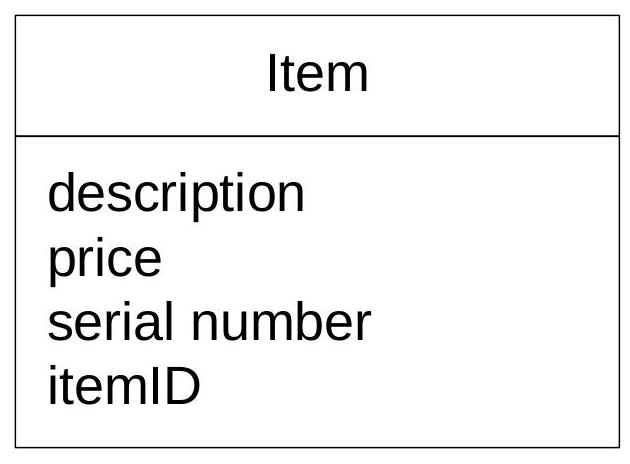
\includegraphics[max width=\textwidth, center]{2025_01_02_5d799754d4e57e7473c6g-21}
\end{itemize}

\section*{Worse}
\begin{center}
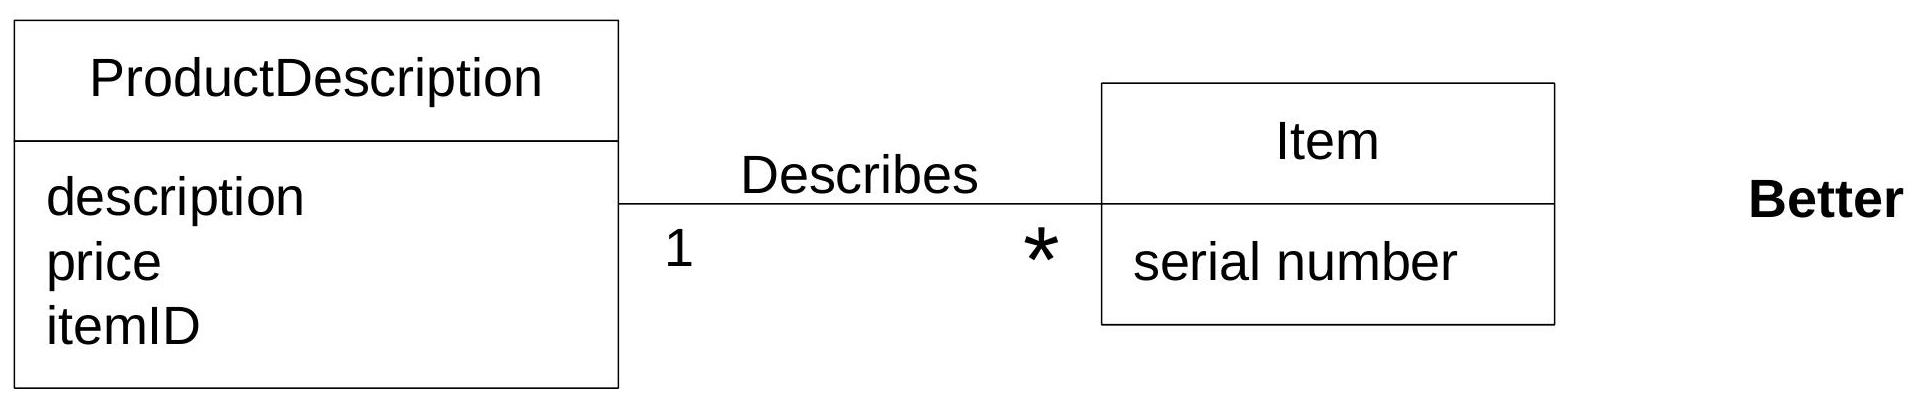
\includegraphics[max width=\textwidth]{2025_01_02_5d799754d4e57e7473c6g-21(1)}
\end{center}

\section*{Generalisierung und Spezialisierung in der Fallstudie}
\begin{itemize}
  \item Es gibt verschiedene Zahlungsmöglichkeiten: Bar, Kreditkarte, Check\\
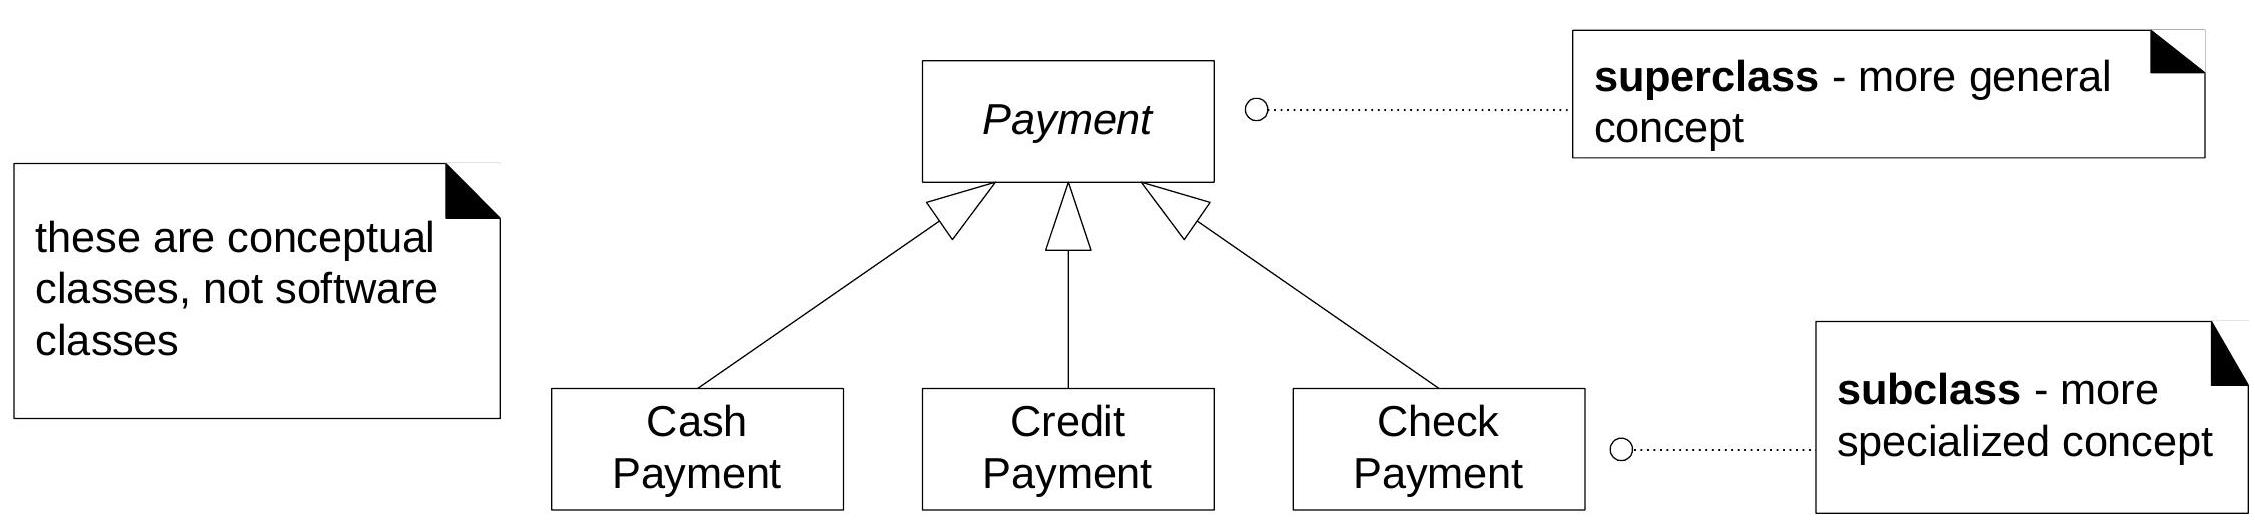
\includegraphics[max width=\textwidth, center]{2025_01_02_5d799754d4e57e7473c6g-22}
\end{itemize}

\section*{Generalisierung und Spezialisierung in der Fallstudie}
\begin{itemize}
  \item Assoziationen und Attribute der generalisierten Klasse werden an die spezialisierten Klassen weitergegeben.\\
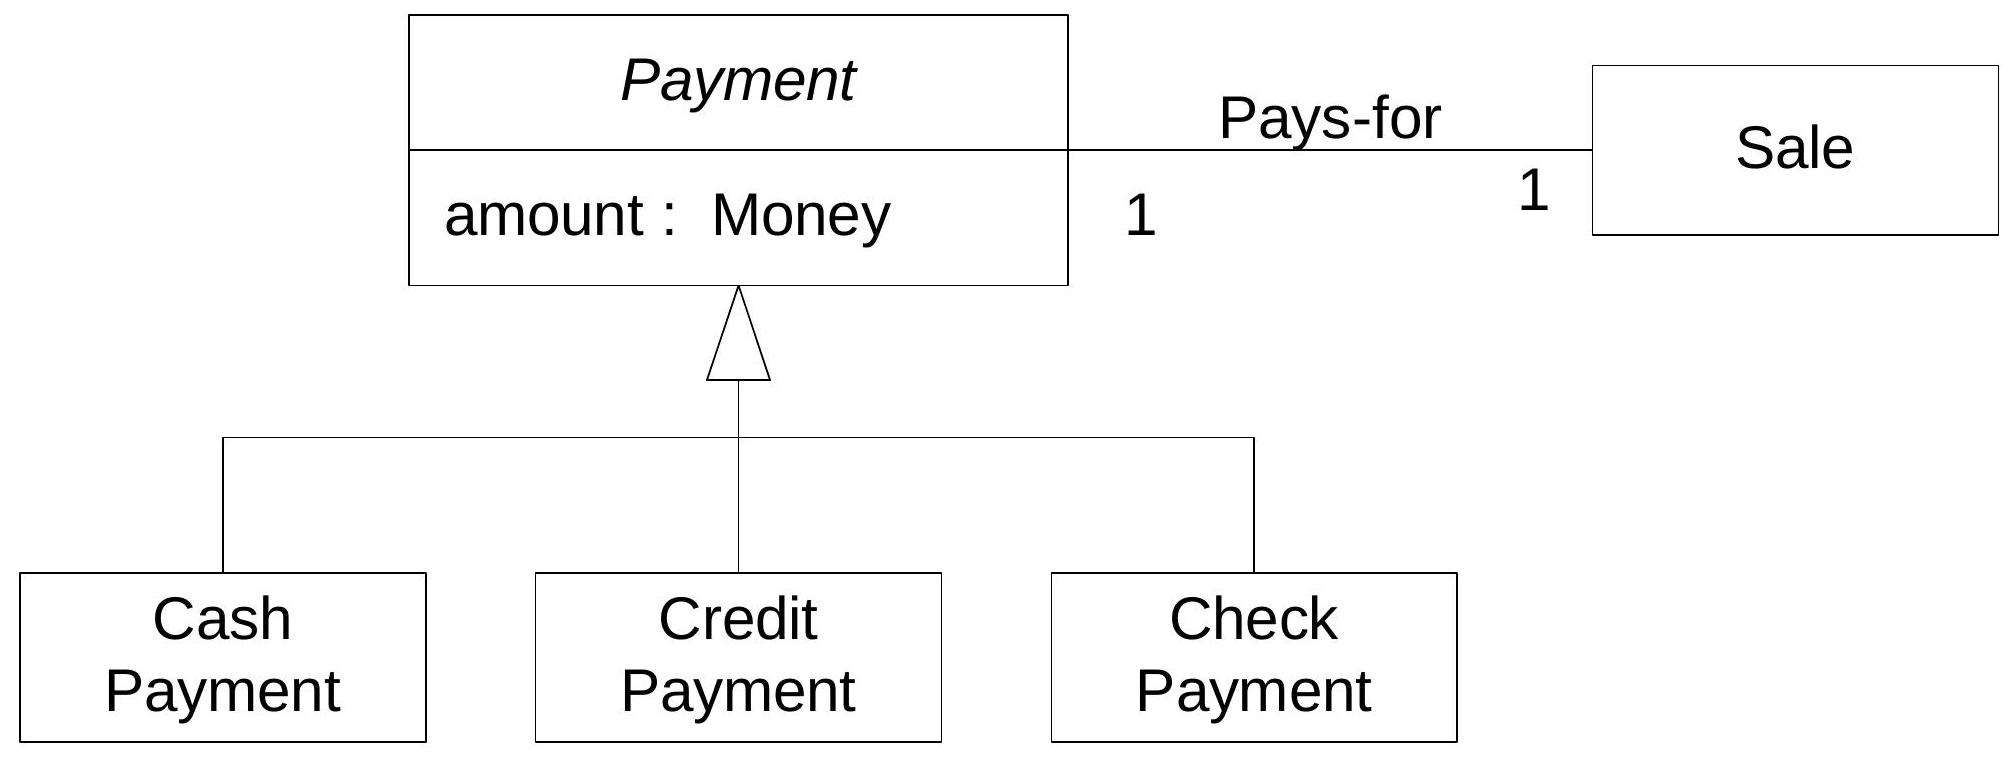
\includegraphics[max width=\textwidth, center]{2025_01_02_5d799754d4e57e7473c6g-23}
\end{itemize}

\section*{Generalisierung und Spezialisierung in der Fallstudie}
School of

\begin{itemize}
  \item Assoziationen und Attribute dienen umgekehrt als Begründung für eine gemeinsame generalisierte Klasse.\\
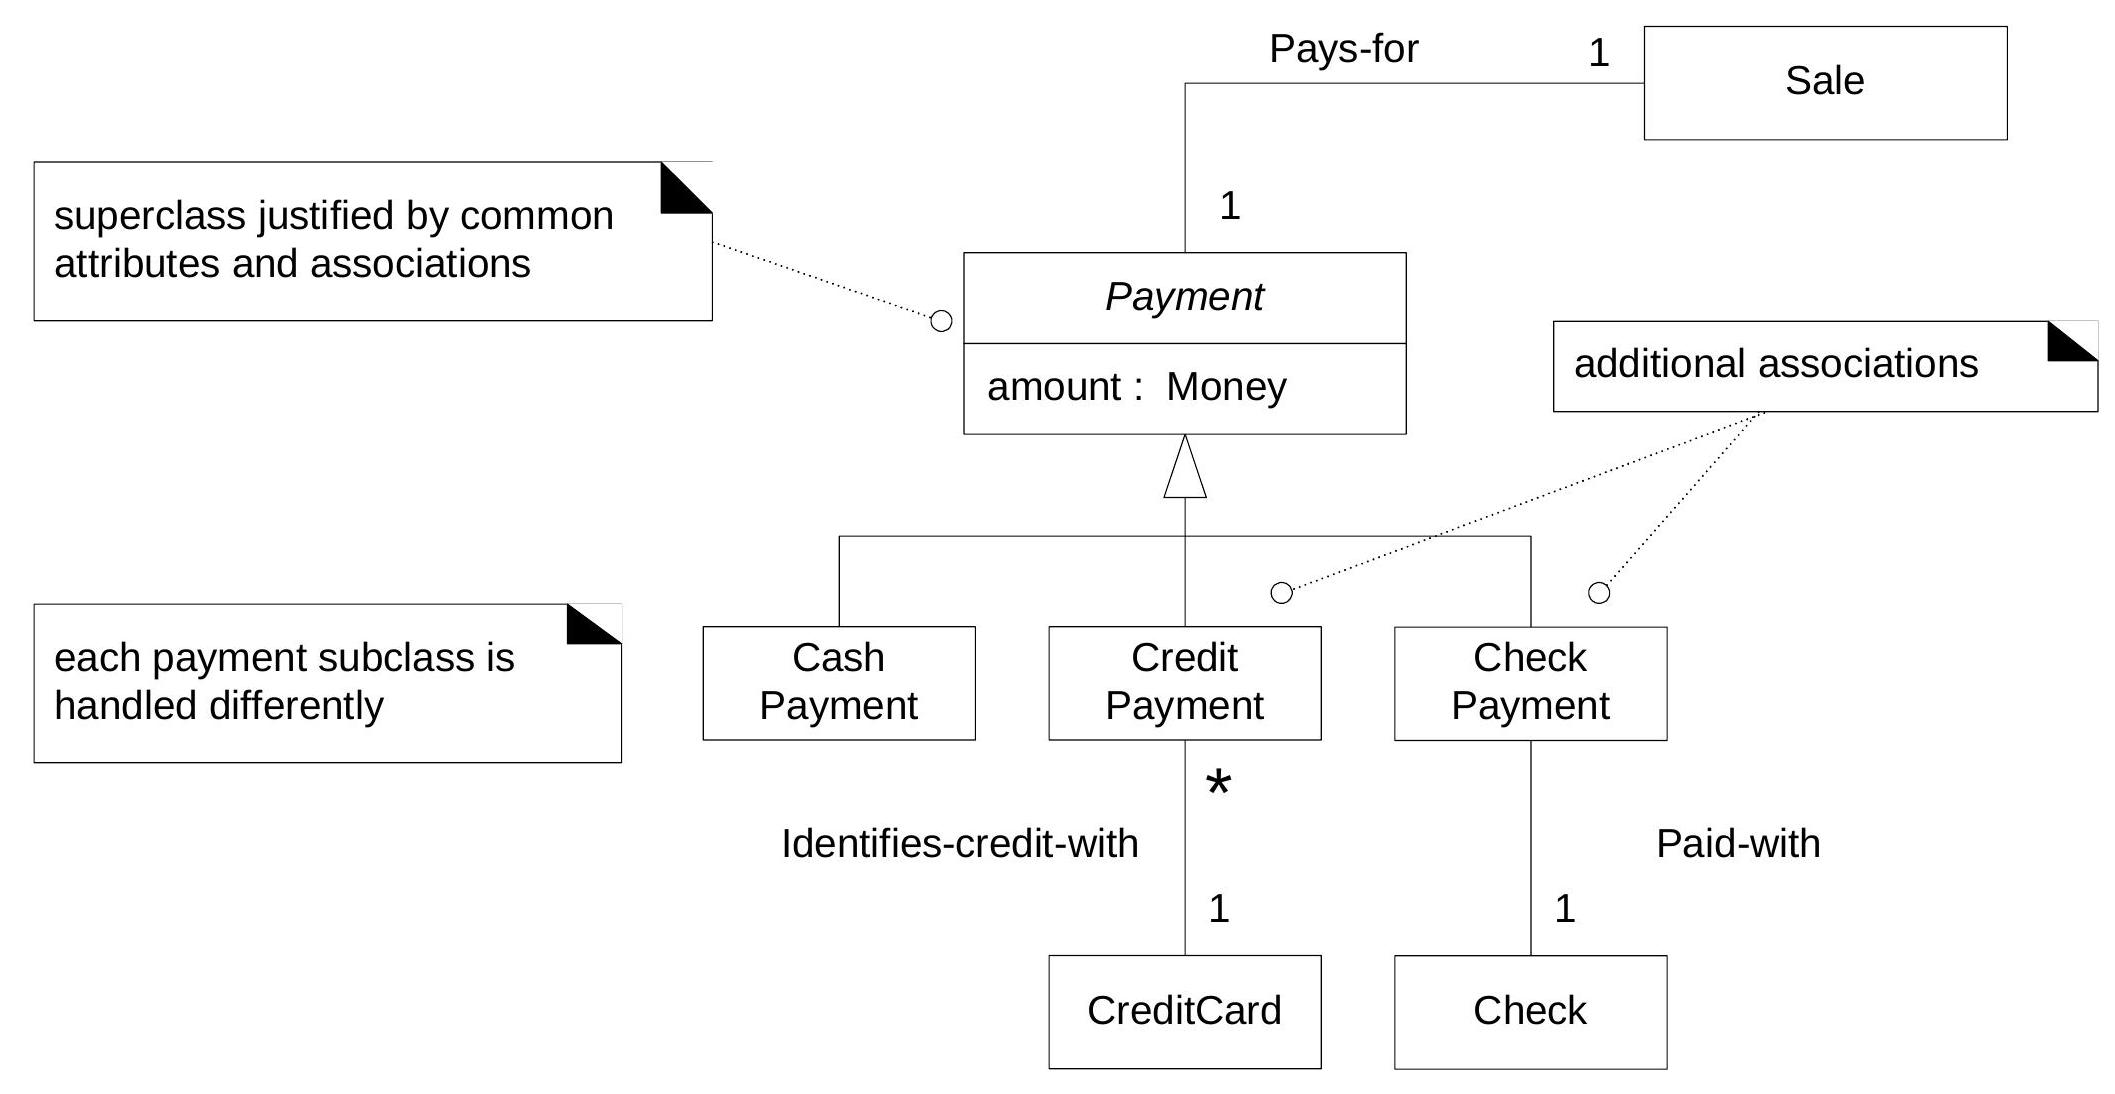
\includegraphics[max width=\textwidth, center]{2025_01_02_5d799754d4e57e7473c6g-24}
\end{itemize}

\section*{Zustände im Domänenmodell}
\begin{itemize}
  \item Verschiedene konkrete und abstrakte Konzepte haben verschiedene Zustände, in denen sie sich befinden.
  \item Naheliegende Lösung
  \item Zustände mittels Spezialisierung modellieren.
  \item Das Problem: Wie können so Zustandsänderungen durchgeführt werden?
  \item Bessere Lösung: Eine eigene Hierarchie für die Zustände definieren.
  \item Diese Lösung entspricht übrigens auch genau dem State-Pattern im SW-Design.\\
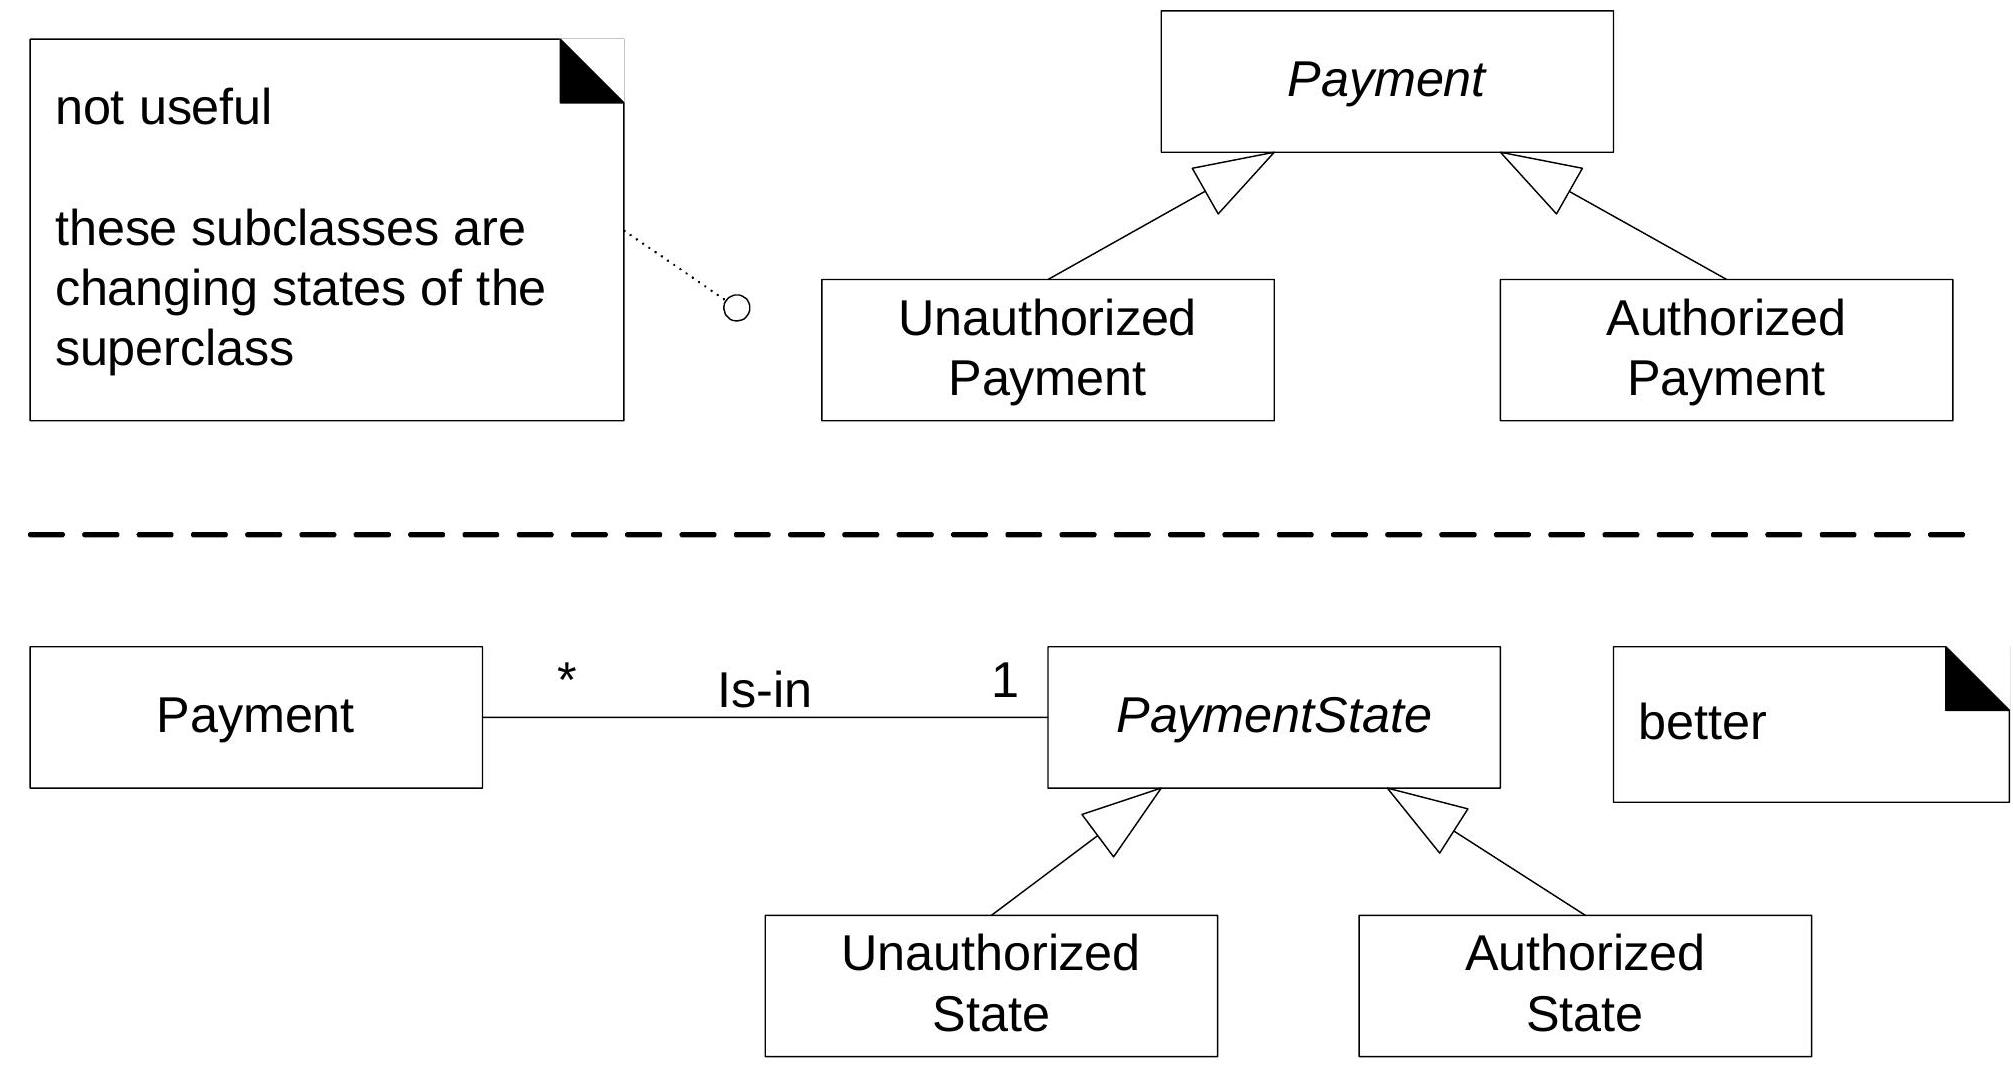
\includegraphics[max width=\textwidth, center]{2025_01_02_5d799754d4e57e7473c6g-26}
\end{itemize}

\section*{Rollen im DM}
\begin{itemize}
  \item Dasselbe Konzept (aber selten dieselbe Instanz) kann unterschiedliche Rollen einnehmen.
  \item Beispiel:
  \item Je nach Stellenprofil hat ein Mitarbeiter andere Aufgaben, allenfalls noch Untergebene.
  \item Eine erste Möglichkeit zur Modellierung
  \item Einsatz einer Assoziation, bei der dann das Ende mit einem Namen versehen wird (siehe nebenan).\\
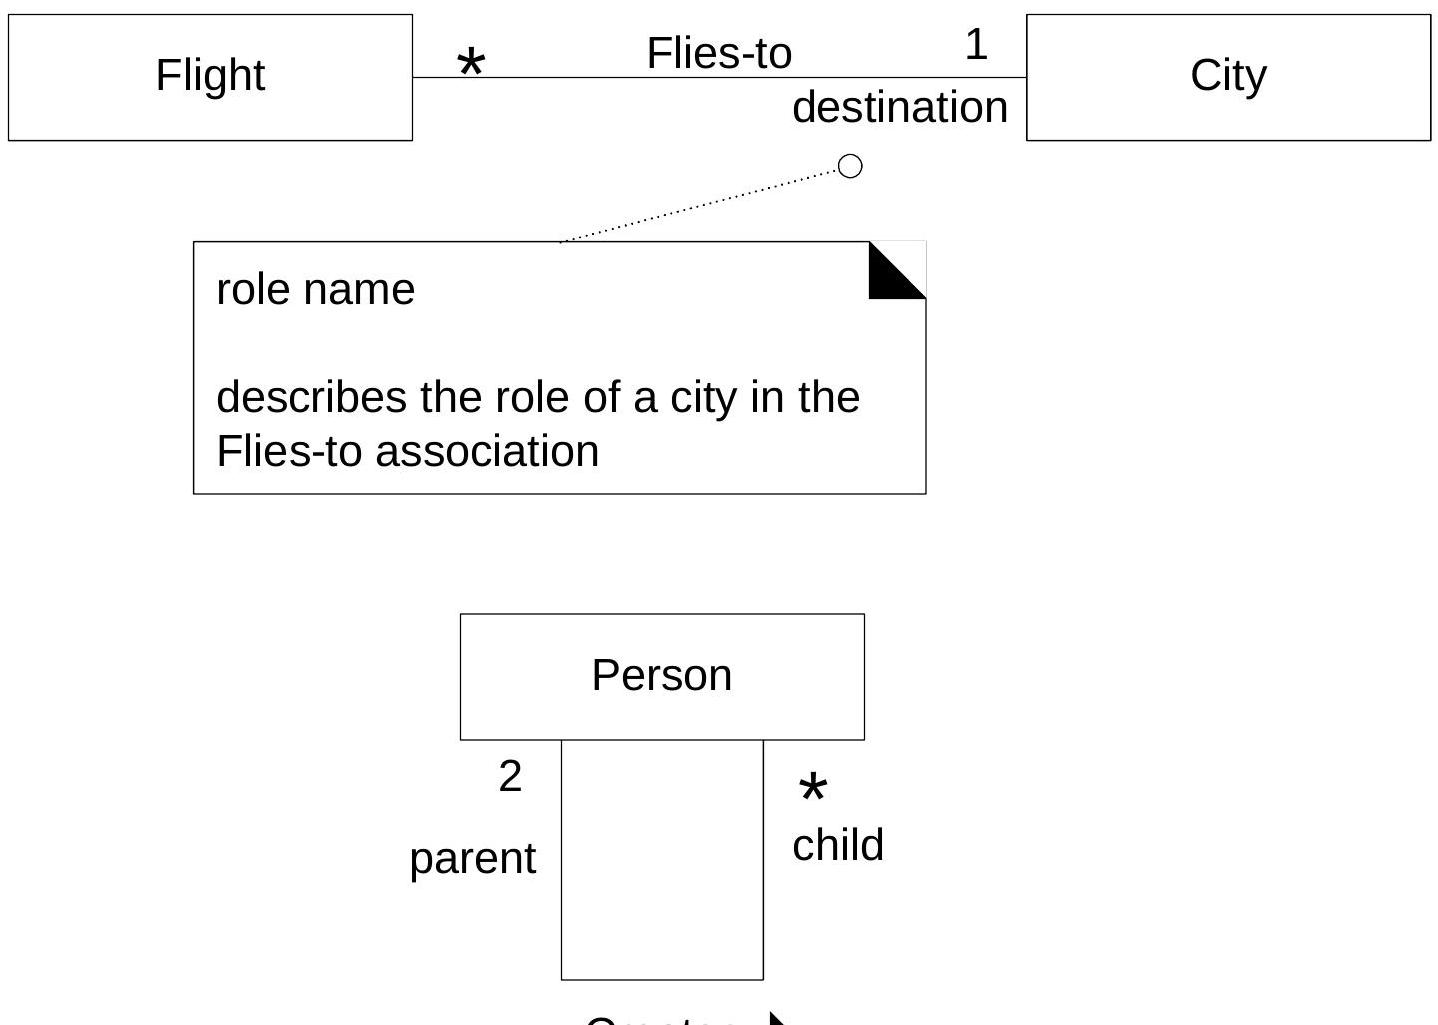
\includegraphics[max width=\textwidth, center]{2025_01_02_5d799754d4e57e7473c6g-27}
\end{itemize}

\section*{Assoziationsklassen}
\begin{itemize}
  \item Pro Kreditkartenherausgeber erhält das Geschäft eine eigene ID, und natürlich hat ein Kreditkartenherausgeber mehr als ein Geschäft als Kunde.
  \item Wo kommt nun diese merchantID hin?
\end{itemize}

\begin{center}
\begin{tabular}{|l|}
\hline
\multicolumn{1}{|c|}{Store} \\
\hline
\begin{tabular}{l}
address \\
merchantID \\
name \\
\end{tabular} \\
\hline
\end{tabular}
\end{center}

$$
\begin{aligned}
& \text { both placements of } \\
& \text { merchantID are incorrect } \\
& \text { because there may be more } \\
& \text { than one merchantID }
\end{aligned}
$$

AuthorizationService\\
address\\
merchantID\\
name\\
phoneNumber

\begin{itemize}
  \item Idee: Genauso, wie n:m Beziehungen mit einer weiteren Klasse zu 2x 1:n aufgebrochen werden, könnte auch hier so eine Klasse eingeführt werden.
  \item Aber eigentlich beschreibt ServiceContract ja die Assoziation zwischen Store und AuthorizationService genauer.\\
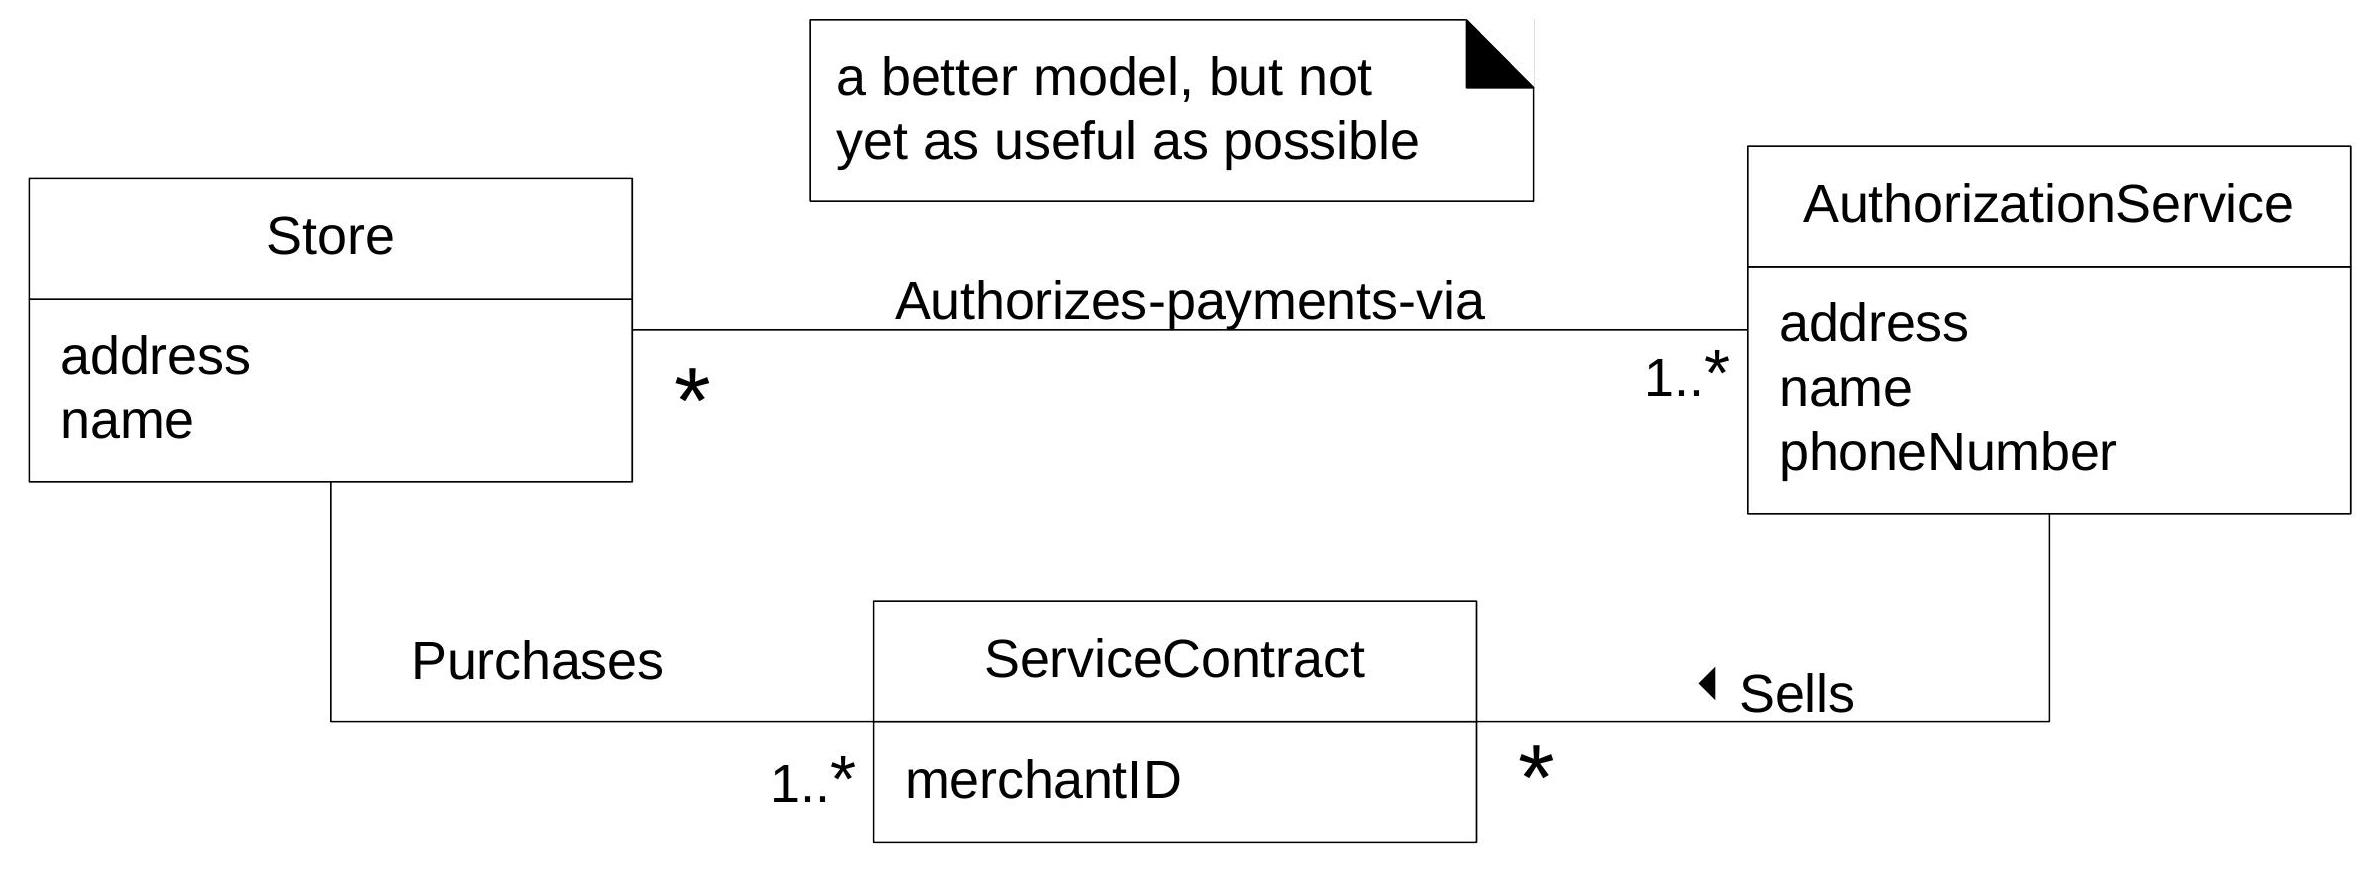
\includegraphics[max width=\textwidth, center]{2025_01_02_5d799754d4e57e7473c6g-29}
\end{itemize}

\section*{Assoziationsklassen}
School of

\begin{itemize}
  \item Für dieses Problem kennt UML eine Lösung: Assoziationsklassen\\
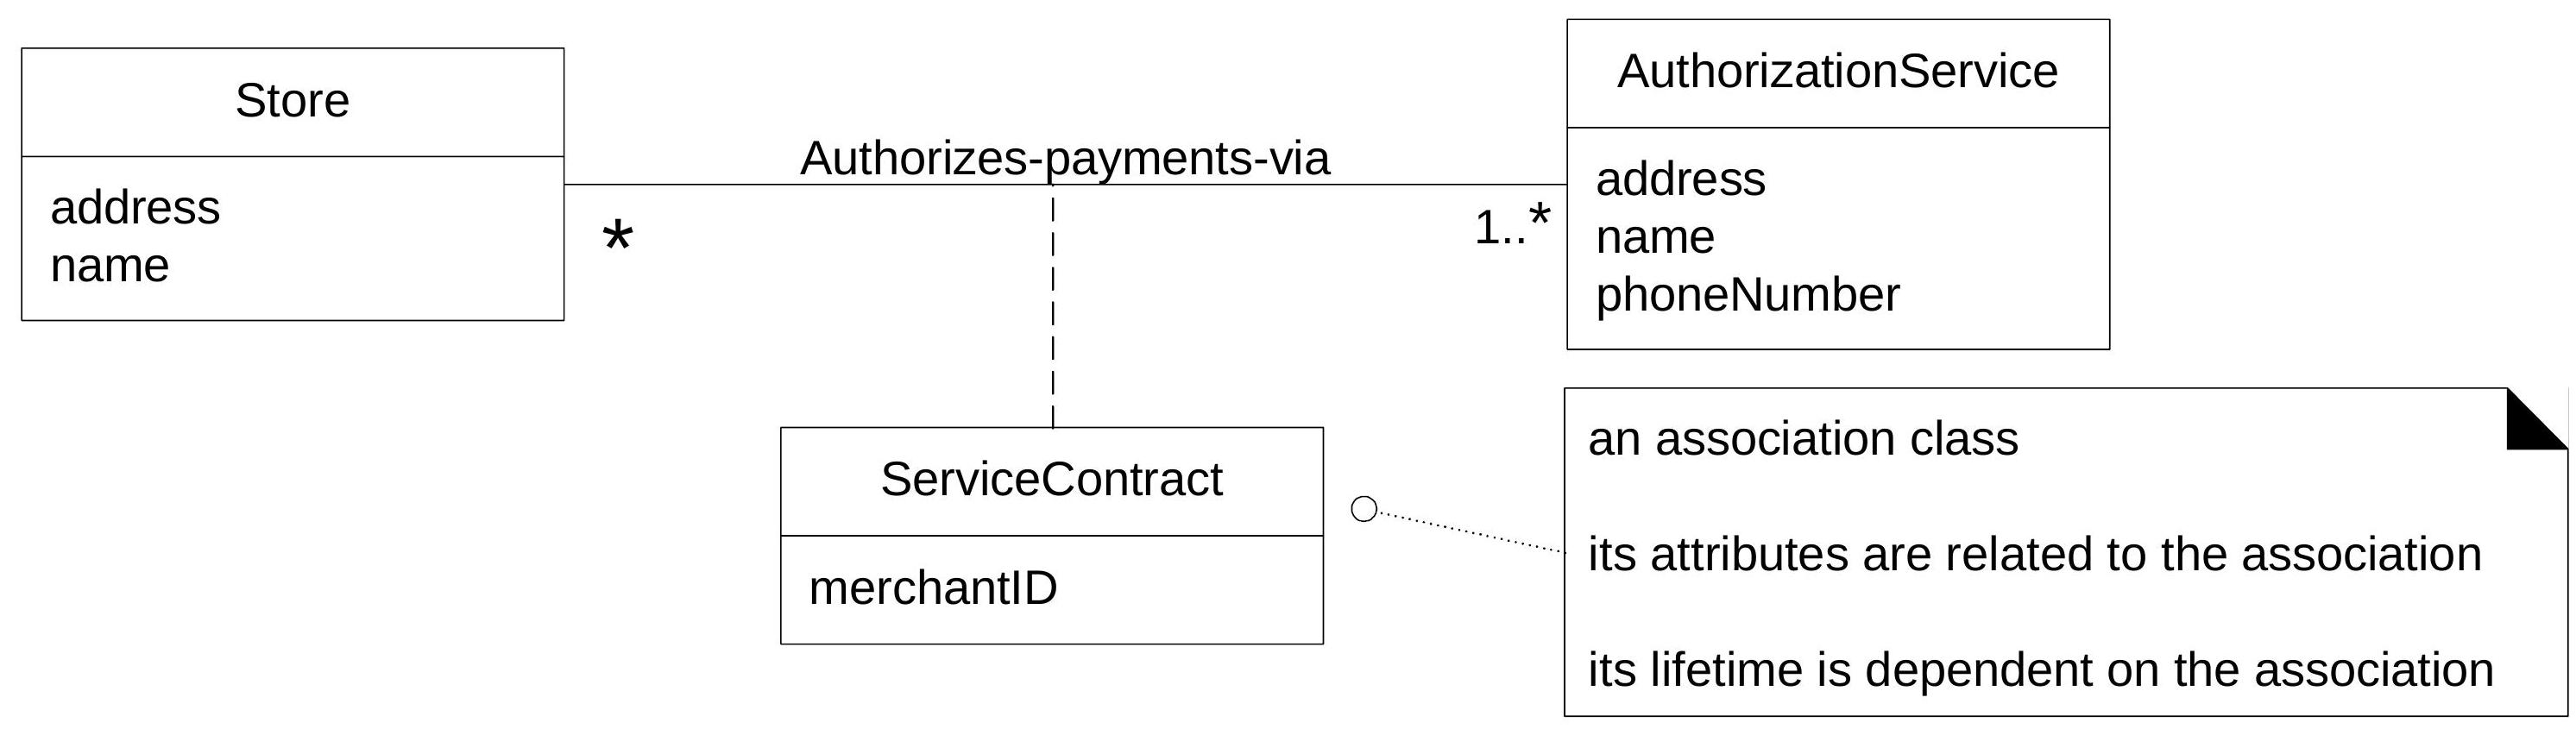
\includegraphics[max width=\textwidth, center]{2025_01_02_5d799754d4e57e7473c6g-30}
  \item Gerade numerische Angaben sind oft mit einer Masseinheit verbunden.
  \item Preis, Gewicht, Volumen, Geschwindigkeit
  \item Ohne Masseinheit kann die angegebene Zahl nicht korrekt interpretiert werden
  \item Häufig macht es Sinn, diese Masseinheit im DM explizit als Konzept zu modellieren.
  \item Money, Weight, Volume
  \item Eine entsprechende SW-Klasse kann später in der Umsetzung noch weitere hilfreiche Methoden aufnehmen
  \item z.B. die Umrechnung von metrischen Werten in imperiale Einheiten.
\end{itemize}

\section*{Agenda}
\begin{enumerate}
  \item Einleitung und Motivation
  \item Grundlagen
  \item Vorgehen
  \item Analysemuster
  \item Wrap-up und Ausblick
\end{enumerate}

\begin{itemize}
  \item Das Domänenmodell visualisiert den Fachbereich in Form eines vereinfachten UML Klassendiagramms.
  \item Das Domänenmodell hilft uns, den Fachbereich zu verstehen und dient als Inspiration für fachliche SW-Klassen.
  \item Entwickeln Sie das Domänenmodell nach denselben Prinzipien, die ein Kartograf einsetzt.
  \item Identifizieren Sie Konzepte, fügen Sie ihnen Attribute hinzu und setzen Sie die Konzepte zueinander in Beziehung.
  \item Wenden Sie bewährte Analysemuster an wie Beschreibungsklassen, Komposition, Generalisierung/Spezialisierung, Zustandsmodellierung und Einheiten als eigene Konzepte.
\end{itemize}

\section*{Ausblick}
\begin{itemize}
  \item In der nächsten Lerneinheit werden wir:
  \item Den Begriff Software Architektur kennenlernen
  \item Verschiedene Softwarearchitekturen genauer anschauen
\end{itemize}

\section*{Quellenverzeichnis}
[1] Larman, C.: UML 2 und Patterns angewendet, mitp Professional, 2005\\[0pt]
[2] Seidel, M. et al.: UML @ Classroom: Eine Einführung in die objektorientierte Modellierung, dpunkt.verlag, 2012


\end{document}